%% Week 45 -- Recurrent neural networks (Chapter 11), built from the earlier
%% course material on RNNs (the FYS5429 lectures on recurrent networks of
%% 2024-2026 and the 2025 week-47 notes, with the Raschka et al. figures
%% RNN1-12 and LSTM1-10 of doc/pub/week47/ipynb/figslides/).  Revised
%% 2026-11-01: all code is TensorFlow/Keras or PyTorch (no NumPy RNN), with
%% frames explaining the two APIs; the theory of Chapter 11 is measured on the
%% library layers with torch.autograd; a spoken-digit demonstration (the Free
%% Spoken Digit Dataset) joins the oscillator, the sine wave, MNIST and the
%% adding problem; one idea per frame.  Figures: week45_*.pdf from
%% make_week45_figures.py, the two TikZ schematics of the book (rnnunroll.pdf,
%% lstmcell.pdf) and the Raschka figures.  The companion notebook
%% week45.ipynb carries all the code.
%% Book references (book.aux 2026-10-25): Chapter 11, Sections 11.1-11.8;
%% Eqs 11.1-11.3 (tasks, chain rule, state space), 11.4 (the RNN), 11.5
%% (cost), 11.6-11.7 (autonomous map, Jacobian), 11.8-11.13 (oscillator),
%% 11.14-11.18 (BPTT), Theorem 11.1 with 11.19-11.20, Corollary 11.2 with
%% 11.21, 11.22 (truncated BPTT), 11.23-11.24 and Proposition 11.3
%% (clipping), 11.25-11.28 (LSTM), 11.29 (cell path), Proposition 11.4 with
%% 11.30-11.31, 11.32 (GRU); Figs 11.1 (unrolled), 11.2 (gradients), 11.3
%% (oscillator), 11.4 (LSTM cell), 11.5 (frameworks); Table 11.1.
%% Build:  pdflatex week45slides.tex  (twice)
\documentclass[10pt,aspectratio=169]{beamer}
\usetheme{red_plain}
\usepackage[T1]{fontenc}
\usepackage[utf8]{inputenc}
\usepackage{amsmath,amssymb,bm}
\usepackage{graphicx}
\usepackage{listings}
\usepackage{xcolor}
\usepackage{booktabs}
\graphicspath{{../BookFigures/chapter11_recurrent_networks/}{../../pub/week47/ipynb/figslides/}{./ch11/}{./figslides/}{./}}

%% ---- code listings
\definecolor{codebg}{rgb}{0.97,0.97,0.97}
\lstset{language=Python,basicstyle=\ttfamily\scriptsize,backgroundcolor=\color{codebg},
  keywordstyle=\color{blue!70!black}\bfseries,commentstyle=\color{green!45!black},
  stringstyle=\color{red!60!black},showstringspaces=false,frame=single,
  framerule=0pt,xleftmargin=4pt,xrightmargin=4pt,breaklines=true,columns=fullflexible}

%% ---- the "pause and think" question frames
\newcounter{insight}
\newenvironment{insight}[1][]{%
  \stepcounter{insight}%
  \begin{frame}{Pause and think \arabic{insight}: #1}%
  \setbeamercolor{block title}{bg=structure.fg,fg=white}%
  \setbeamercolor{block body}{bg=structure.fg!8}%
  \small
}{\end{frame}}
\newcommand{\question}[1]{\begin{block}{Question}#1\end{block}}
\newcommand{\answer}[1]{\pause\begin{block}{Answer}#1\end{block}}

\setbeamertemplate{footline}[frame number]
\setbeamerfont{block title}{size=\small}
\setbeamertemplate{blocks}[rounded][shadow=false]
\setbeamercovered{invisible}



\title{Week 45: Recurrent Neural Networks}
\subtitle{A recap of convolutional networks, then sequences and the hidden
  state, backpropagation through time, why long sequences are hard -- and
  how to do it in TensorFlow/Keras and PyTorch}
\author{Morten Hjorth-Jensen}
\institute{Department of Physics and Center for Computing in Science Education,\\
  University of Oslo, Norway}
\date{}

\begin{document}

\begin{frame}
\titlepage
\end{frame}

\begin{frame}{Plan for week 45}
\small
\textbf{Monday lecture (2$\times$45 min):}
\begin{enumerate}
  \item \textbf{Recap of convolutional networks} (15 min): what week 44
        established, and the Keras and PyTorch programs for MNIST.
  \item \textbf{From feed-forward to recurrent networks}: what we give up,
        what a sequence model is asked to do, the hidden state.
  \item \textbf{The architecture}: the simple RNN, folded and unrolled;
        the RNN as a dynamical system; where the recurrence comes from.
  \item \textbf{The layers in Keras and PyTorch}: what \texttt{SimpleRNN}
        and \texttt{nn.RNN} compute, line by line.
  \item \textbf{Backpropagation through time}: the recursion, and what
        \texttt{loss.backward()} does with it.
  \item \textbf{Why long sequences are hard}: vanishing and exploding
        gradients, measured with autograd; clipping; a network that learns
        the rule of a damped oscillator.
  \item \textbf{Three applications}: a sine wave, MNIST row by row, and
        the adding problem -- where the simple RNN runs out of memory.
\end{enumerate}
\medskip
\textbf{Next Monday, first hour:} gated cells (LSTM, GRU) and sound.\\
\textbf{Tuesday:} work on Project 2 (deadline \textbf{Monday November 9});
no weekly exercises this week.\\
\textbf{Reading:} Chapter 11, Sections 11.1--11.6 and 11.8; Chapter 10 for
the recap.  The code is in \texttt{week45.ipynb}.
\end{frame}

%% =====================================================================
\section{Recap: convolutional networks}
\begin{frame}{Recap of week 44, 1: what a CNN is}
Convolutional networks are ordinary neural networks with one assumption
built into the architecture: \emph{the input is an image}.
\begin{itemize}
  \item Neurons with learnable weights and biases, dot products and
        non-linearities; one differentiable function from pixels to class
        scores; the softmax cross entropy at the end; trained by
        backpropagation and Adam.  Nothing new there.
  \item \textbf{What is new:} each neuron sees only a small region of the
        input -- its receptive field -- and the \emph{same} weights (a
        filter) are applied at every position.
\end{itemize}
\begin{block}{Two consequences}
Far fewer parameters than a dense layer, independent of the image size;
and a pattern learned once is recognised wherever it appears (shift
equivariance, Theorem 10.7).
\end{block}
\end{frame}

\begin{frame}{Recap of week 44, 2: the convolution stage}
For an input volume $W_1\times H_1\times D_1$ and $K$ filters of size
$F\times F$ with stride $S$ and padding $P$, each output pixel is a dot
product of a filter with a window of the input (cross-correlation,
Chapter 10):
\[
  z_{i,j,k}=b_k+\sum_{c=1}^{D_1}\sum_{u=1}^{F}\sum_{v=1}^{F}
  w_{u,v,c,k}\;x_{Si+u,\,Sj+v,\,c}.
\]
\begin{columns}[T]
\begin{column}{0.5\textwidth}
\begin{block}{The output volume}
\[
  W_2=\frac{W_1-F+2P}{S}+1,\qquad D_2=K
\]
(and the same for $H_2$).
\end{block}
\end{column}
\begin{column}{0.46\textwidth}
\begin{block}{Parameters}
$(F\times F\times D_1)\times K+K$: for MNIST with $32$ filters of
$3\times3$, $320$ -- whatever the image size.
\end{block}
\end{column}
\end{columns}
\medskip
Pooling (a fixed $2\times2$ maximum or average) halves width and height
between convolution stages; ReLU follows each convolution.
\end{frame}

\begin{frame}{Recap of week 44, 3: the network we ran (Raschka et al.)}
\begin{center}
\includegraphics[width=0.85\textwidth]{deepcnn}
\end{center}
Convolution -- pooling -- convolution -- pooling -- flatten -- dense --
dense: $28\times28\times1\to28\times28\times32\to14\times14\times32
\to14\times14\times64\to7\times7\times64\to1024\to10$, with $3\times3$
filters.  Keras wants the data as $(N,28,28,1)$, channels \emph{last};
PyTorch as $(N,1,28,28)$, channels \emph{first}.
\end{frame}

\begin{frame}[fragile]{Recap of week 44, 4: the Keras program}
\begin{lstlisting}[basicstyle=\ttfamily\tiny]
model = keras.Sequential([
    keras.Input(shape=(28, 28, 1)),
    layers.Conv2D(32, 3, padding="same", activation="relu"),  # 28x28x32, 320 parameters
    layers.MaxPooling2D((2, 2)),                              # 14x14x32
    layers.Conv2D(64, 3, padding="same", activation="relu"),  # 14x14x64, 18496
    layers.MaxPooling2D((2, 2)),                              # 7x7x64
    layers.Flatten(),                                         # 3136
    layers.Dense(1024, activation="relu"),                    # 3212288
    layers.Dropout(0.5),
    layers.Dense(10)])                                        # 10250, logits
model.compile(optimizer=keras.optimizers.Adam(1e-3),
              loss=keras.losses.SparseCategoricalCrossentropy(from_logits=True),
              metrics=["accuracy"])
model.fit(Xtr, ytr, epochs=5, batch_size=64)
\end{lstlisting}
\small
\begin{itemize}
  \item \texttt{Conv2D(K, F, padding="same")}: $K$ filters of $F\times F$,
        padded so that the size is kept; \texttt{MaxPooling2D((2, 2))}
        halves it.
  \item \texttt{from\_logits=True}: the network ends with scores and the
        loss applies the softmax itself.  \texttt{Dropout(0.5)}
        regularises the layer that holds $99\%$ of the parameters.
  \item The pattern \texttt{Sequential} -- \texttt{compile} -- \texttt{fit}
        is the one we will use for recurrent layers today.
\end{itemize}
\end{frame}

\begin{frame}[fragile]{Recap of week 44, 5: the same network in PyTorch}
\begin{lstlisting}[basicstyle=\ttfamily\tiny]
net = nn.Sequential(
    nn.Conv2d(1, 32, 3, padding=1), nn.ReLU(), nn.MaxPool2d(2, 2),   # (N,32,14,14)
    nn.Conv2d(32, 64, 3, padding=1), nn.ReLU(), nn.MaxPool2d(2, 2),  # (N,64,7,7)
    nn.Flatten(), nn.Linear(64 * 7 * 7, 1024), nn.ReLU(),
    nn.Dropout(0.5), nn.Linear(1024, 10))                            # logits
opt, lossf = torch.optim.Adam(net.parameters(), lr=1e-3), nn.CrossEntropyLoss()
for epoch in range(5):
    net.train()                                   # dropout on
    for idx in torch.randperm(len(Xtr)).split(64):
        opt.zero_grad()
        loss = lossf(net(Xtr[idx]), Ytr[idx])
        loss.backward()                           # backpropagation, by autograd
        opt.step()
    net.eval()                                    # dropout off for the test accuracy
\end{lstlisting}
\small
\begin{itemize}
  \item \texttt{nn.Conv2d(C\_in, K, F, padding=P)}: input channels, filters,
        filter size, padding.
  \item PyTorch shows the loop that \texttt{fit} hides: minibatch, loss,
        \texttt{backward()}, a step of Adam.  The same loop, unchanged,
        trains every recurrent network today.
  \item \texttt{nn.CrossEntropyLoss} expects logits; \texttt{train()} /
        \texttt{eval()} switch dropout on and off.
\end{itemize}
\end{frame}

\begin{frame}{Recap of week 44, 6: what we found on MNIST}
\begin{center}
\small
\begin{tabular}{@{}llrc@{}}
\toprule
code & model & parameters & test accuracy\\
\midrule
PyTorch & dense 784--100--10 (Project 2) & $79\,510$ & $0.9720$\\
Keras & dense 784--100--10 & $79\,510$ & $0.9720$\\
PyTorch & CNN of the listings & $3\,241\,354$ & $0.9906$\\
Keras & CNN of the listings & $3\,241\,354$ & $0.9909$\\
PyTorch & CNN with global average pooling & $19\,466$ & $0.9336$\\
Keras & CNN with global average pooling & $19\,466$ & $0.9398$\\
\bottomrule
\end{tabular}

\medskip
\footnotesize Five epochs, Adam $10^{-3}$, batches of $64$, seed $1$; full
curves in \texttt{week44\_mnist.pdf}.
\end{center}
\begin{itemize}
  \item The CNN makes $94$ errors on the $10\,000$ test images where the
        Project 2 dense network makes $280$; the two libraries agree to the
        noise of a stochastic optimiser.
  \item On the scikit-learn digits placed at a random position the dense
        network lost $26$ points and the CNN $9$: convolution pays when
        patterns can appear \emph{anywhere on a grid}.
\end{itemize}
\end{frame}

\begin{frame}{From space to time}
\begin{block}{Week 44}
A filter does not care how large the image is, and finds a pattern wherever
it is: \emph{parameter sharing along the spatial axes}.
\end{block}
\begin{block}{Today}
A recurrent cell does not care how long the sequence is, and applies the
same update at every step: \emph{parameter sharing along the time axis}.
\end{block}
\medskip
Same idea, same consequences -- a parameter count independent of the input
size, and equivariance (to shifts in space, to shifts in time) -- and, as we
will see, a new difficulty that convolution does not have: the sharing is
\emph{recursive}, each step feeding the next.
\end{frame}

%% =====================================================================
\section{From feed-forward to recurrent networks}


\begin{frame}{What we have assumed so far, 1: independent samples}
Almost everything since week 35 -- the bias-variance decomposition, the
bootstrap, cross-validation, the statistical toolbox of Chapter 2 -- leans
on the training examples being \emph{independent and identically
distributed}.

\medskip
For a sequence this is simply false.  The value of a detector trace at one
sample is strongly informative about the next; that is the entire content
of the data.

\medskip
\begin{block}{The consequence}
A model that treats the samples as independent has thrown the signal away
before it starts.
\end{block}
\end{frame}

\begin{frame}{What we have assumed so far, 2: a fixed input size}
A feed-forward network has a fixed input dimension.  A convolutional
network (week 44) has one too, up to the pooling that precedes its dense
layers.

\medskip
Sequences come in different lengths -- a measurement that ran for ten
seconds and one that ran for an hour, a spoken word of $0.3$ s and one of
$0.6$ s -- and we would like \emph{one} model to handle all of them.
\end{frame}

\begin{frame}{The move of this chapter}
\begin{block}{Week 44}
We restricted the dense layer so that it respects the \emph{spatial}
structure of an image, and obtained \emph{convolution}.
\end{block}
\begin{block}{Today}
We make the same kind of restriction for data with a \emph{temporal}
structure, and obtain \emph{recurrence}: process one element at a time and
carry a state forward, so that the same parameters serve a sequence of any
length.
\end{block}
\end{frame}

\begin{frame}{Sequences in the physical sciences}
Ordered, correlated data are the norm rather than the exception:
\begin{itemize}
  \item detector read-out streams and waveform traces;
  \item climate and seismic records;
  \item molecular-dynamics trajectories and spectroscopy scans;
  \item state estimation in control and feedback;
  \item the solutions of differential equations, which are time series by
        construction;
  \item sound and speech (next Monday).
\end{itemize}
\medskip
Sequential need not mean temporal (text, genomes), but our examples are
time series.  We write $x_{1:T}=(\bm{x}_1,\dots,\bm{x}_T)$.
\end{frame}

\begin{frame}{Three tasks, Eq.~(11.1)}
\begin{columns}[T]
\begin{column}{0.5\textwidth}
\[
  p(x_{1:T}),\qquad p(y_{1:T}\mid x_{1:T}),\qquad p(y\mid x_{1:T}).
\]
\begin{itemize}
  \item modelling the sequence itself;
  \item mapping a sequence to a sequence: filtering, forecasting
        (\emph{many-to-many});
  \item mapping a sequence to one label: classification, regime detection
        (\emph{many-to-one}).
\end{itemize}
\medskip
Today: the oscillator is many-to-many; the sine wave, MNIST and the adding
problem are many-to-one.
\end{column}
\begin{column}{0.48\textwidth}
\begin{center}
\includegraphics[width=0.8\textwidth]{RNN5}\\
\scriptsize Figures in this part from Raschka and Mirjalili, \emph{Python
Machine Learning}.
\end{center}
\end{column}
\end{columns}
\end{frame}

\begin{frame}{What is a recurrent neural network?}
\begin{columns}[T]
\begin{column}{0.46\textwidth}
In a feed-forward network the information flows in one direction only,
from the input to the output.

\medskip
A recurrent network also has connections pointing \emph{backward}: the
hidden layer is connected to \emph{itself}.  The hidden state at step $t$
receives two inputs -- the data $\bm{x}^{(t)}$ and its own value
$\bm{h}^{(t-1)}$ from the previous step.

\medskip
\begin{block}{What this buys}
A \emph{memory} across time steps, and the same layer for the first element
of a sequence and the thousandth.
\end{block}
\end{column}
\begin{column}{0.52\textwidth}
\begin{center}
\includegraphics[width=\textwidth]{RNN1}
\end{center}
\end{column}
\end{columns}
\end{frame}

\begin{frame}{Fold and unfold: two drawings of the same computation}
\begin{center}
\includegraphics[width=0.6\textwidth]{RNN2}
\end{center}
\begin{columns}[T]
\begin{column}{0.48\textwidth}
\begin{block}{Folded (left)}
A single layer with an arrow leaving it and returning to itself.  This is
how the network is \emph{stored}: one copy of the weights.
\end{block}
\end{column}
\begin{column}{0.48\textwidth}
\begin{block}{Unrolled (right)}
The same layer drawn once per time step.  This is how the network is
\emph{executed} -- and, as we will see, how it is \emph{differentiated}.
\end{block}
\end{column}
\end{columns}
\end{frame}

\begin{frame}{The hidden state: a latent state-space model}
The chain rule of probability factorises the first task exactly, Eq.~(11.2),
\[
  p(x_{1:T}) = \prod_{t=1}^{T} p\!\left(\bm{x}_t \mid x_{1:t-1}\right),
\]
exact and useless as it stands: the conditioning set grows without bound.
What makes it tractable is the assumption that everything relevant in
$x_{1:t-1}$ can be summarised in a finite-dimensional \emph{state}
$\bm{h}_t$, updated recursively, Eq.~(11.3):
\[
  \boxed{\;\bm{h}_t = f_\theta\!\left(\bm{h}_{t-1},\bm{x}_t\right),\qquad
  \hat{\bm{y}}_t = g_\theta\!\left(\bm{h}_t\right).\;}
\]
\begin{block}{This should look familiar}
Equation~(11.3) is the structure of a \emph{Markovian dynamical system}.
The Kalman filter is the case where $f_\theta$ is linear and the noise
Gaussian.  A recurrent neural network is the case where $f_\theta$ and
$g_\theta$ are neural networks -- the update map is \emph{learned}.
\end{block}
\end{frame}


%% =====================================================================
\section{The architecture}


\begin{frame}{The simple RNN, Eq.~(11.4)}
\begin{columns}[T]
\begin{column}{0.5\textwidth}
One affine map and one activation per step:
\[
\begin{aligned}
  \bm{a}^{(t)} &= \bm{U}\bm{x}^{(t)} + \bm{W}\bm{h}^{(t-1)} + \bm{b},\\
  \bm{h}^{(t)} &= \sigma_h\!\left(\bm{a}^{(t)}\right),\\
  \bm{o}^{(t)} &= \bm{V}\bm{h}^{(t)} + \bm{c},\\
  \hat{\bm{y}}^{(t)} &= \sigma_y\!\left(\bm{o}^{(t)}\right),
\end{aligned}
\]
$\bm{U}\in\mathbb{R}^{n_h\times n_x}$ maps the input into the state,
$\bm{W}\in\mathbb{R}^{n_h\times n_h}$ the state to itself,
$\bm{V}\in\mathbb{R}^{n_y\times n_h}$ reads the state out; $\bm{h}^{(0)}=\bm{0}$.

\medskip
$\sigma_h$ is almost always $\tanh$ (Part 6 says why); $\sigma_y$ is the
identity for regression, the softmax for classification.
\end{column}
\begin{column}{0.48\textwidth}
\begin{center}
\includegraphics[width=\textwidth]{RNN8}\\
\scriptsize Raschka's notation: $\bm{U}=\bm{W}_{hx}$, $\bm{W}=\bm{W}_{hh}$,
$\bm{V}=\bm{W}_{yh}$.
\end{center}
\end{column}
\end{columns}
\end{frame}

\begin{frame}{The same arrays at every step (Figure 11.1)}
\begin{center}
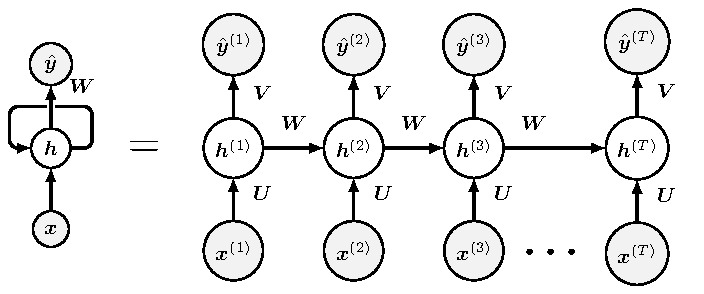
\includegraphics[width=0.55\textwidth]{rnnunroll}
\end{center}
\begin{block}{The parameters do not depend on $t$}
Parameter sharing along the time axis, exactly as convolution shares
parameters along the spatial axes (week 44): the parameter count is
independent of the sequence length, and the model is equivariant to a shift
in time.
\end{block}
\end{frame}

\begin{frame}{Two more properties of Eq.~(11.4)}
\begin{block}{The state is a bottleneck}
Everything the network will ever know about $x_{1:t}$ when it predicts
$\hat{\bm{y}}^{(t+1)}$ must fit in the $n_h$ numbers of $\bm{h}^{(t)}$.
\end{block}
\begin{block}{The cost accumulates over the sequence, Eq.~(11.5)}
\[
  \mathcal{L}=\frac1T\sum_{t=1}^{T}L^{(t)},\qquad
  L^{(t)}=\tfrac12\|\hat{\bm{y}}^{(t)}-\bm{y}^{(t)}\|^2
\]
for regression, the cross entropy for classification.  In the
sequence-to-label case only $L^{(T)}$ is non-zero -- the hardest case of
all, as Part 6 will show.
\end{block}
\end{frame}

\begin{frame}{Stacking: a multilayer RNN}
\begin{columns}[T]
\begin{column}{0.42\textwidth}
The hidden state of one recurrent layer can be the input sequence of the
next.  Each layer has its own $\bm{U},\bm{W},\bm{b}$ and is unrolled along
the same time axis, so the unrolled graph becomes a grid: depth in layers
downwards, depth in time sideways.

\medskip
In the libraries: \texttt{num\_layers=2} in \texttt{nn.RNN}, or two
\texttt{SimpleRNN} layers with \texttt{return\_sequences=True} in Keras
(Part 4).
\end{column}
\begin{column}{0.56\textwidth}
\begin{center}
\includegraphics[width=\textwidth]{RNN3}
\end{center}
\end{column}
\end{columns}
\end{frame}

\begin{frame}{The RNN as a discrete-time dynamical system (Section 11.2.1)}
Set the input to zero.  Equation~(11.4) becomes an autonomous map,
Eq.~(11.6),
\[
  \bm{h}^{(t)} = F\!\left(\bm{h}^{(t-1)}\right)
  := \sigma_h\!\left(\bm{W}\bm{h}^{(t-1)}+\bm{b}\right).
\]
Fixed points satisfy $\bm{h}^\star=F(\bm{h}^\star)$; their stability is
decided by the Jacobian, Eq.~(11.7),
\[
  \bm{J}=\left.\frac{\partial F}{\partial\bm{h}}\right|_{\bm{h}^\star}
  =\operatorname{diag}\!\left(\sigma_h'(\bm{a}^\star)\right)\bm{W},
\]
attracting if the spectral radius $\rho(\bm{J})<1$, repelling if
$\rho(\bm{J})>1$.  In two dimensions the map can have limit cycles, in three
or more it can be chaotic.
\end{frame}

\begin{frame}{Why this matters, twice}
\begin{block}{What a recurrent network can represent}
Oscillations, decay to a point attractor, chaotic wandering.
\end{block}
\begin{block}{What it does with information}
Strongly contracting dynamics forget the initial condition quickly and
cannot carry information far; expanding dynamics are unstable.
\end{block}
\medskip
Equation~(11.7) is also exactly the quantity that will control the gradient
in Part 6: the stability of the forward dynamics and the survival of the
backward gradient are the \emph{same question}.
\end{frame}

\begin{frame}{The one-dimensional map, and an untrained \texttt{nn.RNN} (\texttt{week45\_dynamics.pdf})}
\begin{center}
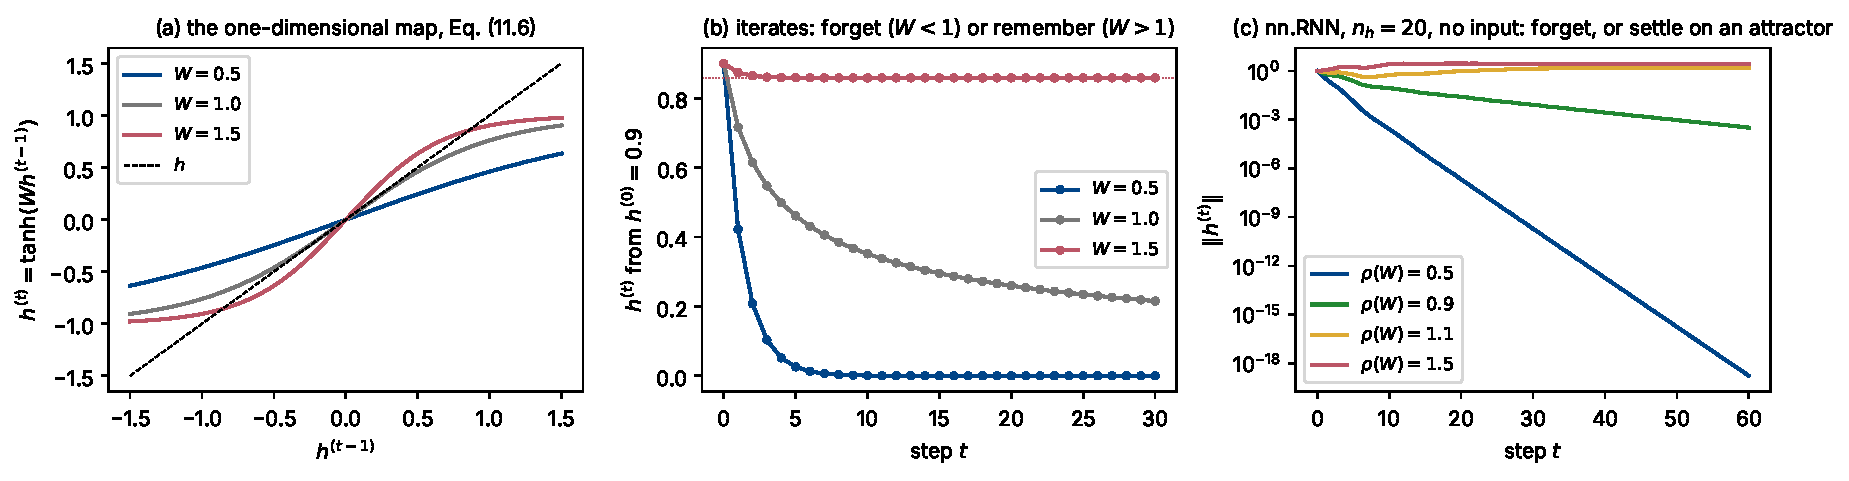
\includegraphics[width=\textwidth]{week45_dynamics}
\end{center}
\small
(a) $h\mapsto\tanh(Wh)$ against the diagonal: for $W<1$ the only fixed point
is $0$, for $W>1$ two new ones appear.  (b) Iterates from $h^{(0)}=0.9$: at
$W=0.5$ the state is gone after ten steps, at $W=1.5$ it sits on
$h^\star=\pm0.8586$ for ever.  (c) A PyTorch \texttt{nn.RNN} with $n_h=20$,
zero input, $\bm{W}$ scaled to a given spectral radius: at $\rho(\bm{W})=0.5$
the norm of the state falls by nineteen orders of magnitude in sixty steps;
at $\rho>1$ it settles on an attractor of order one.
\end{frame}


%% =====================================================================
\section{Where the recurrence comes from}


\begin{frame}{A differential equation (Section 11.3)}
The recurrence of Eq.~(11.4) can look arbitrary.  It is not.  Newton's
equation for a damped harmonic oscillator, scaled to dimensionless time,
Eq.~(11.8):
\[
  \frac{\mathrm{d}^2x}{\mathrm{d}t^2}+\eta\frac{\mathrm{d}x}{\mathrm{d}t}+x(t)=F(t),
\]
with $\eta$ the damping and $F$ an external force.  As always we rewrite it
as two coupled first-order equations, Eq.~(11.9),
\[
  v=\frac{\mathrm{d}x}{\mathrm{d}t},\qquad
  \frac{\mathrm{d}v}{\mathrm{d}t}=F(t)-\eta v(t)-x(t),
\]
and integrate from $(x_0,v_0)$ -- by hand for $F=0$, by Runge-Kutta in
general.
\end{frame}

\begin{frame}{Discretise, and the recurrence appears}
Forward Euler for the velocity gives step $i+1$ from step $i$, Eq.~(11.10):
\[
  v_{i+1}=v_i+\Delta t\left(F_i-\eta v_i-x_i\right)=:h_i\!\left(x_i,v_i,F_i\right),
\]
a function of the \emph{current state} and the \emph{current input}.  But
$v_i$ was itself produced by the same rule one step earlier, Eq.~(11.11),
so substituting, Eq.~(11.12), and renaming, Eq.~(11.13),
\[
  v_{i+1}=h_i\!\left(x_i,\,h_{i-1},\,F_i\right)
  \qquad\Longrightarrow\qquad
  \bm{h}_i=h\!\left(\bm{x}_i,\bm{h}_{i-1}\right),
\]
which is Eq.~(11.3) exactly.
\end{frame}

\begin{frame}{A recurrent network is a learned, non-linear time-stepper}
\begin{block}{The correspondence}
\begin{itemize}
  \item the hidden state plays the role of the integrator's internal state;
  \item $\bm{W}$ plays the role of $1-\eta\Delta t$;
  \item the training data supply what the differential equation would
        otherwise have to tell us.
\end{itemize}
\end{block}
\medskip
The output $\hat{y}_i$ is compared with a target through a cost -- the
target being a measurement, or the solution of the equation.
\end{frame}

\begin{frame}{The data for today's experiment (\texttt{week45\_oscillator\_data.pdf})}
\begin{center}
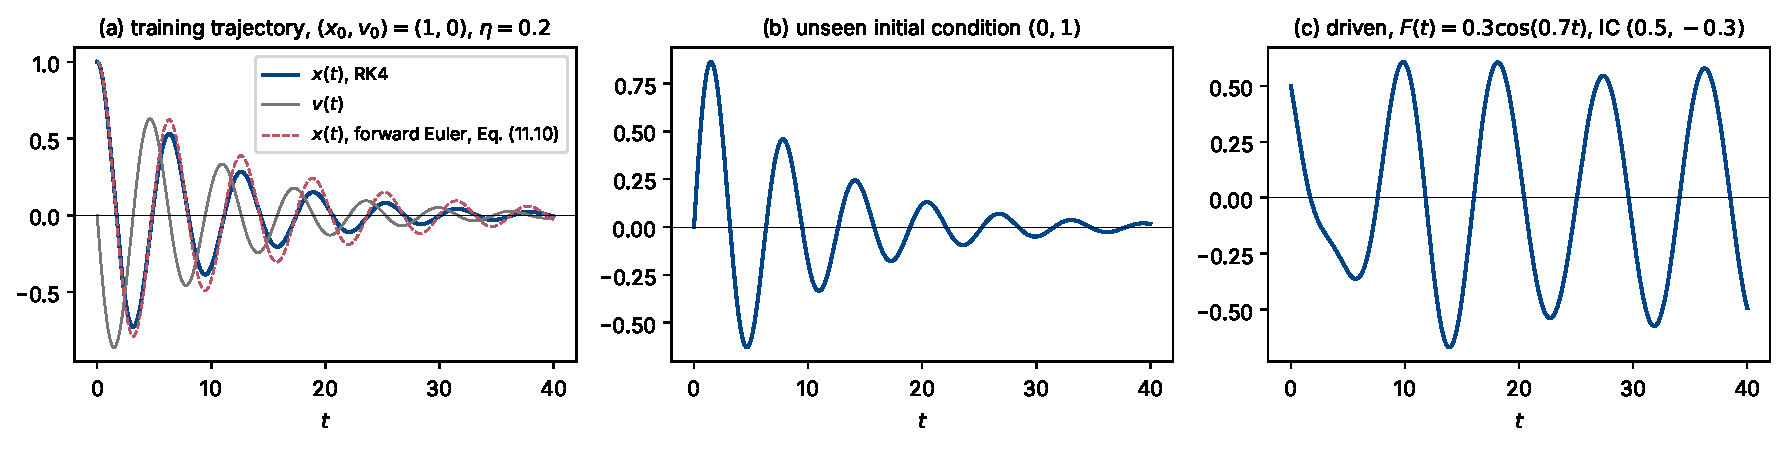
\includegraphics[width=\textwidth]{week45_oscillator_data}
\end{center}
\small
Fourth-order Runge-Kutta with $\eta=0.2$ on $t\in[0,40]$, $800$ points.
Forward Euler at the same $\Delta t=0.05$ (dashed) is visibly off by the
second period -- an error of $0.1$ -- a first hint of what a \emph{learned}
stepper can improve on.  In Part 6 the network sees only the blue curve of
(a); (b) and (c) are the tests.
\end{frame}

\begin{frame}{Compare week 42: two ways to solve a differential equation with a network}
\begin{columns}[T]
\begin{column}{0.48\textwidth}
\begin{block}{Chapter 9 (week 42)}
The equation was \emph{known} and supplied the cost through its residual;
no data were needed; the network learned a function of continuous time.
\end{block}
\end{column}
\begin{column}{0.48\textwidth}
\begin{block}{Chapter 11 (today)}
The equation is \emph{unknown} and the data supply the cost; the network
learns a discrete update rule.
\end{block}
\end{column}
\end{columns}
\medskip
The first is for known physics and absent data, the second for present data
and unknown physics.
\end{frame}


%% =====================================================================
\section{The layers in Keras and PyTorch}


\begin{frame}{Two libraries, one layer}
\begin{center}
\footnotesize
\begin{tabular}{lll}
\toprule
Equation & TensorFlow/Keras & PyTorch\\
\midrule
simple RNN, Eq.~(11.4) & \texttt{layers.SimpleRNN(units)} & \texttt{nn.RNN(input\_size, hidden\_size)}\\
gated cells (next Monday) & \texttt{layers.LSTM}, \texttt{layers.GRU} & \texttt{nn.LSTM}, \texttt{nn.GRU}\\
read-out $\bm{V}\bm{h}+\bm{c}$ & \texttt{layers.Dense(n\_y)} & \texttt{nn.Linear(hidden\_size, n\_y)}\\
clipping, Eq.~(11.23) & \texttt{Adam(lr, clipnorm=1.0)} & \texttt{nn.utils.clip\_grad\_norm\_(params, 1.0)}\\
BPTT & inside \texttt{model.fit} & \texttt{loss.backward()}\\
\bottomrule
\end{tabular}
\end{center}
\begin{block}{The one convention to remember: the data layout}
Both libraries want a 3-tensor of shape \texttt{(samples, timesteps,
features)} $=(N,T,n_x)$: $N$ sequences, each $T$ steps of $n_x$ numbers.
In PyTorch this needs \texttt{batch\_first=True} (the default is
$(T,N,n_x)$).  A single time series is \emph{cut into windows} to make the
first axis.
\end{block}
\end{frame}

\begin{frame}[fragile]{Keras: a minimal recurrent model}
\begin{lstlisting}
from tensorflow import keras
from tensorflow.keras import layers

model = keras.Sequential([
    keras.Input(shape=(None, 1)),               # (T, n_x): T may vary, one feature per step
    layers.SimpleRNN(24, return_sequences=True), # Eq. (11.4): h_t for every t, n_h = 24
    layers.Dense(1),                             # V h_t + c, applied at every step
])
model.compile(optimizer=keras.optimizers.Adam(5e-3, clipnorm=1.0), loss="mse")
model.summary()                                  # 24*(1+24+1) + 25 = 649 parameters
history = model.fit(X_train, Y_train, epochs=300, batch_size=4, verbose=0)
\end{lstlisting}
\small
\texttt{X\_train} has shape $(N,T,1)$ and \texttt{Y\_train} the shape
$(N,T,1)$ of the targets -- here one target per step, the
sequence-to-sequence case.  Six lines; the next frame reads them one by one.
\end{frame}

\begin{frame}{Keras: what each line does}
\small
\begin{description}
  \item[\texttt{Input(shape=(None, 1))}] the shape of \emph{one} sample
        without the batch axis: $T$ steps (\texttt{None} = any length) of
        $n_x=1$ features.
  \item[\texttt{SimpleRNN(24)}] one recurrent layer with $n_h=24$: $\bm{U}$
        ($1\times24$, stored transposed as \texttt{kernel}), $\bm{W}$
        ($24\times24$, \texttt{recurrent\_kernel}), $\bm{b}$ (\texttt{bias});
        $\tanh$ by default; $\bm{h}^{(0)}=\bm{0}$.
  \item[\texttt{return\_sequences=True}] output all of $\bm{h}^{(1)},\dots,\bm{h}^{(T)}$,
        shape $(N,T,24)$.  With \texttt{False} (the default) only
        $\bm{h}^{(T)}$, shape $(N,24)$ -- the sequence-to-label case.
  \item[\texttt{Dense(1)}] $\bm{V}\bm{h}+\bm{c}$.  Applied to a 3-tensor it
        acts on the last axis, i.e.\ at every time step with the same
        $\bm{V},\bm{c}$.
  \item[\texttt{compile(...)}] the optimiser (Adam, week 38) and the cost;
        \texttt{clipnorm=1.0} is gradient clipping, Eq.~(11.23), on the whole
        gradient vector.
  \item[\texttt{fit(...)}] forward pass, backpropagation through time and the
        update, \texttt{epochs} times over all windows in mini-batches of
        \texttt{batch\_size} windows.
\end{description}
\end{frame}

\begin{frame}{Keras: the knobs you will actually use}
\small
\begin{itemize}
  \item \texttt{SimpleRNN} $\to$ \texttt{LSTM} $\to$ \texttt{GRU} (next
        Monday): change one word; the shapes of input and output are the
        same.
  \item \texttt{return\_sequences=True} on every layer but the last to
        \emph{stack} recurrent layers; \texttt{return\_state=True} to also
        get the final state.
  \item \texttt{Input(shape=(T, n\_x))} with a fixed $T$ when all windows
        have the same length (faster); \texttt{None} when they do not.
  \item Variable-length sequences in one batch: pad, and put a
        \texttt{layers.Masking(mask\_value=0.0)} first so that padded steps
        are skipped.
  \item Classification from the last state: \texttt{Dense(n\_classes)}
        with \texttt{SparseCategoricalCrossentropy(from\_logits=True)} --
        the softmax and the cross entropy of week 41 in one object.
\end{itemize}
\end{frame}

\begin{frame}[fragile]{PyTorch: the same model}
\begin{lstlisting}
import torch, torch.nn as nn

class Forecaster(nn.Module):
    def __init__(self, n_h=24):
        super().__init__()
        self.rnn = nn.RNN(input_size=1, hidden_size=n_h, batch_first=True)  # Eq. (11.4), tanh
        self.fc = nn.Linear(n_h, 1)                                         # V h_t + c

    def forward(self, x):                   # x: (N, T, 1)
        H, h_T = self.rnn(x)                # H: (N, T, n_h) = every h_t;  h_T: (1, N, n_h)
        return self.fc(H)                   # (N, T, 1): one prediction per step

model = Forecaster()
print(sum(p.numel() for p in model.parameters()))   # 673 (two bias vectors, see below)
\end{lstlisting}
\small
PyTorch separates the \emph{definition} of the network (a class with a
\texttt{forward}) from its \emph{training} (a loop you write).  Keras hides
the loop in \texttt{fit}; PyTorch shows it -- which is why we use it when we
want to see the gradients.
\end{frame}

\begin{frame}{PyTorch: what each line does}
\small
\begin{description}
  \item[\texttt{nn.RNN(input\_size, hidden\_size, batch\_first=True)}]
        Eq.~(11.4) with $\tanh$ (\texttt{nonlinearity="relu"} is the other
        option).  \texttt{batch\_first=True} makes the input $(N,T,n_x)$.
        \texttt{num\_layers=2} stacks two layers.
  \item[\texttt{self.rnn(x)} returns a pair] \texttt{H} of shape $(N,T,n_h)$
        with all hidden states, and \texttt{h\_T} of shape
        $(\texttt{num\_layers},N,n_h)$ with the last one.  You choose: all of
        \texttt{H} for sequence-to-sequence, \texttt{H[:, -1, :]} for
        sequence-to-label.
  \item[the parameters] \texttt{weight\_ih\_l0} is $\bm{U}$ ($n_h\times n_x$),
        \texttt{weight\_hh\_l0} is $\bm{W}$, and there are \emph{two} biases
        \texttt{bias\_ih\_l0} and \texttt{bias\_hh\_l0} whose sum is our
        $\bm{b}$ -- hence $673=649+24$.
  \item[\texttt{nn.Linear(n\_h, 1)}] $\bm{V}\bm{h}+\bm{c}$ on the last axis,
        exactly like Keras's \texttt{Dense}.
  \item[\texttt{nn.LSTM}, \texttt{nn.GRU}] (next Monday) same calls, same
        shapes.
\end{description}
\end{frame}

\begin{frame}[fragile]{PyTorch: the training loop, line by line}
\begin{lstlisting}
opt = torch.optim.Adam(model.parameters(), lr=5e-3)
lossfn = nn.MSELoss()
for epoch in range(300):
    for idx in torch.randperm(len(X_train)).split(4):        # shuffle windows, batches of 4
        opt.zero_grad()                                        # forget last batch's gradients
        loss = lossfn(model(X_train[idx]), Y_train[idx])      # forward pass, Eq. (11.5)
        loss.backward()                                        # BPTT, Eqs. (11.16)-(11.18)
        gnorm = nn.utils.clip_grad_norm_(model.parameters(), 1.0)   # Eq. (11.23); returns ||g||
        opt.step()                                             # Adam update, week 38
\end{lstlisting}
\small
\begin{itemize}
  \item \texttt{randperm(...).split(4)}: the \emph{windows} are shuffled,
        the time order inside each window is not.
  \item \texttt{zero\_grad()}: PyTorch \emph{accumulates} gradients into
        \texttt{.grad}, so each batch starts by clearing them.
  \item \texttt{loss.backward()}: automatic differentiation through the
        unrolled graph -- Part 5 says what it computes.
  \item \texttt{clip\_grad\_norm\_} rescales the whole gradient in place if
        its norm exceeds $1$ and returns the norm \emph{before} clipping --
        which is how we will look at it.
\end{itemize}
\end{frame}

\begin{frame}[fragile]{Counting parameters in both libraries}
\begin{lstlisting}
 layer                 Keras   PyTorch   formula n_h(n_x+n_h+1)      n_x=1, n_h=24
 SimpleRNN / nn.RNN      624       648       624
 + Dense(1) / Linear      25        25        25   (n_y(n_h+1))
 whole model             649       673
\end{lstlisting}
\small
\begin{itemize}
  \item Keras's \texttt{SimpleRNN} prints exactly Eq.~(11.4):
        $n_h(n_x+n_h+1)=24\cdot26=624$.  Use \texttt{model.summary()} as a
        check of what you built.
  \item PyTorch is larger by $n_h$: the second bias vector.  The model is
        the same, only the parameterisation is redundant.
  \item Neither count contains $T$.  A dense network fed the flattened
        window of $T=40$ values with $24$ hidden nodes has $1009$ parameters,
        and $9649$ at $T=400$ -- and must be retrained when $T$ changes.
\end{itemize}
\end{frame}

\begin{frame}[fragile]{Same weights, same outputs: the conventions (Section 11.8.3)}
\begin{lstlisting}
rnn = nn.RNN(n_x, n_h, batch_first=True)                 # PyTorch, random weights
U = rnn.weight_ih_l0.detach().numpy()                     # (n_h, n_x)
W = rnn.weight_hh_l0.detach().numpy()                     # (n_h, n_h)
b = (rnn.bias_ih_l0 + rnn.bias_hh_l0).detach().numpy()    # one bias in Eq. (11.4)
k = keras.Sequential([keras.Input(shape=(T, n_x)), layers.SimpleRNN(n_h, return_sequences=True)])
k.layers[0].set_weights([U.T, W.T, b])                    # Keras stores the transposes
print(np.max(np.abs(rnn(X)[0].detach().numpy() - k(X.numpy()).numpy())))   # 1.2e-07
\end{lstlisting}
\small
Two conventions differ: PyTorch has two biases where Eq.~(11.4) has one,
and Keras stores $\bm{U}$ and $\bm{W}$ transposed (\texttt{kernel} is
$(n_x,n_h)$).  With those reconciled the hidden states agree to $10^{-7}$
-- single precision -- for the same inputs: the two libraries compute the
same function, and it is Eq.~(11.4).
\end{frame}


%% =====================================================================
\section{Backpropagation through time}


\begin{frame}{Training: unroll, and backpropagate (Section 11.4)}
\small
\begin{columns}[T]
\begin{column}{0.5\textwidth}
\begin{block}{The idea}
A recurrent network run for $T$ steps \emph{is} a feed-forward network of
depth $T$ in which every layer shares the same weights.  Backpropagation
(week 41) applies unchanged; the only novelty is that the gradients from
every step must be \emph{summed} into the same parameter arrays.
\end{block}
\begin{block}{In the time domain}
\begin{enumerate}
  \item The forward pass builds a \emph{stack} of the activities at each
        time step.
  \item The backward pass peels the stack to compute the error derivatives
        at each time step.
  \item The derivatives at all times are added together for each weight.
\end{enumerate}
\end{block}
\end{column}
\begin{column}{0.48\textwidth}
\begin{center}
\includegraphics[width=0.92\textwidth]{RNN9}\\
\scriptsize The red arrows are the backward pass; the loss is a sum over
time (Werbos 1990).
\end{center}
\end{column}
\end{columns}
\end{frame}

\begin{frame}{The output layer and the last hidden state}
Differentiating the cost (11.5) gives, for each $t$, Eq.~(11.14),
\[
  \left(\nabla_{\bm{o}^{(t)}}\mathcal{L}\right)_i
  =\frac{\partial\mathcal{L}}{\partial L^{(t)}}
   \frac{\partial L^{(t)}}{\partial o_i^{(t)}},
\]
which for the quadratic cost and a linear $\sigma_y$ is simply
$(\hat{\bm{y}}^{(t)}-\bm{y}^{(t)})/T$ -- the output error of week 41, divided
by the number of steps.

\medskip
At $t=T$ the state influences the cost \emph{only} through the output at
that step, Eq.~(11.15):
\[
  \nabla_{\bm{h}^{(T)}}\mathcal{L}=\bm{V}^{\mathsf{T}}\nabla_{\bm{o}^{(T)}}\mathcal{L}.
\]
This is where the backward pass starts: at the last step, with nothing
arriving from the future.
\end{frame}

\begin{frame}{Earlier hidden states have two routes to the cost}
For $t<T$ the state $\bm{h}^{(t)}$ reaches the cost through the output at
step $t$ \emph{and} through the state at step $t+1$.  The chain rule gives
two terms, Eq.~(11.16),
\[
  \boxed{\;
  \nabla_{\bm{h}^{(t)}}\mathcal{L}
  =\left(\frac{\partial\bm{h}^{(t+1)}}{\partial\bm{h}^{(t)}}\right)^{\!\mathsf{T}}
   \nabla_{\bm{h}^{(t+1)}}\mathcal{L}
  +\left(\frac{\partial\bm{o}^{(t)}}{\partial\bm{h}^{(t)}}\right)^{\!\mathsf{T}}
   \nabla_{\bm{o}^{(t)}}\mathcal{L}\;}
\]
and with Eq.~(11.4) the two Jacobians are explicit, Eq.~(11.17):
\[
  \nabla_{\bm{h}^{(t)}}\mathcal{L}
  =\bm{W}^{\mathsf{T}}\operatorname{diag}\!\left(\sigma_h'(\bm{a}^{(t+1)})\right)
   \nabla_{\bm{h}^{(t+1)}}\mathcal{L}
  +\bm{V}^{\mathsf{T}}\nabla_{\bm{o}^{(t)}}\mathcal{L}.
\]
Equations (11.15) and (11.17), run backwards from $t=T$ to $t=1$, are the
whole of backpropagation through time.
\end{frame}

\begin{frame}{Compare week 41}
\begin{block}{The first term}
is the $\delta$-recursion of Eq.~(8.64): $\bm{W}^{\mathsf{T}}$ times the
error of the next layer times the derivative of the activation -- with
``next layer'' meaning ``next time step'' and the same $\bm{W}$ at every
step.
\end{block}
\begin{block}{The second term}
is new: every layer of the unrolled network has its own output and its own
piece of the cost.
\end{block}
\end{frame}

\begin{frame}{The parameters: every step contributes, Eq.~(11.18)}
Because the same matrices act at every step, each accumulates a contribution
from every step.  With
$\bm{\delta}^{(t)}=\operatorname{diag}(\sigma_h'(\bm{a}^{(t)}))\,\nabla_{\bm{h}^{(t)}}\mathcal{L}$,
\[
\begin{aligned}
  \nabla_{\bm{c}}\mathcal{L}&=\sum_t\nabla_{\bm{o}^{(t)}}\mathcal{L}, &
  \nabla_{\bm{V}}\mathcal{L}&=\sum_t\left(\nabla_{\bm{o}^{(t)}}\mathcal{L}\right)\bm{h}^{(t)\mathsf{T}},\\
  \nabla_{\bm{b}}\mathcal{L}&=\sum_t\bm{\delta}^{(t)}, &
  \nabla_{\bm{W}}\mathcal{L}&=\sum_t\bm{\delta}^{(t)}\bm{h}^{(t-1)\mathsf{T}}, &
  \nabla_{\bm{U}}\mathcal{L}&=\sum_t\bm{\delta}^{(t)}\bm{x}^{(t)\mathsf{T}}.
\end{aligned}
\]
Each term is the week-41 formula ``error times the input of that layer'',
Eqs.~(8.67)--(8.68); the sum over $t$ is the weight sharing.
\end{frame}

\begin{frame}{The backward pass is linear}
There is an asymmetry between the two passes that is easy to miss.
\begin{block}{Forward}
Non-linear: $\sigma_h$ squashes, which keeps the activities bounded and is
what prevents them from exploding.
\end{block}
\begin{block}{Backward}
\emph{Completely linear} in the incoming gradient: Eq.~(11.16) is a matrix
acting on $\nabla_{\bm{h}^{(t+1)}}\mathcal{L}$, the matrix fixed by the
forward pass.  Double the error at the final step and every derivative
doubles.
\end{block}
\medskip
Nothing bounds the backward pass, which is precisely why it can explode
when the forward pass cannot.
\end{frame}

\begin{frame}[fragile]{What \texttt{loss.backward()} computes}
We do not write Eqs.~(11.15)--(11.18) ourselves: both libraries record the
unrolled graph during the forward pass and differentiate it backwards --
reverse-mode automatic differentiation (week 38).  Two consequences:
\begin{itemize}
  \item the gradient is \emph{exactly} the recursion above, to rounding;
  \item it is a fixed linear map of the output error, which we can test:
\end{itemize}
\begin{lstlisting}
rnn, fc = nn.RNN(2, 6, batch_first=True).double(), nn.Linear(6, 1).double()
for scale in (1.0, 2.0):                       # output error e, then 2e
    for q in params: q.grad = None
    loss = 0.5 * ((fc(rnn(X)[0]) - target(scale)) ** 2).sum()
    loss.backward()                            # BPTT
    grads.append([q.grad.clone() for q in params])
# max |g(2e) - 2 g(e)| / max|g(2e)| = 4.3e-16         (float64: exact)
\end{lstlisting}
\small In Keras the same thing happens inside \texttt{model.fit}; to see it,
use \texttt{tf.GradientTape()} around the forward pass and call
\texttt{tape.gradient(loss, model.trainable\_variables)}.
\end{frame}

\begin{frame}{What travels backwards in the sequence-to-label case}
Suppose the cost is non-zero only at the last step ($L^{(t)}=0$ for $t<T$:
a label for the whole window, \texttt{H[:, -1, :]} or
\texttt{return\_sequences=False}).  Then the second term of Eq.~(11.16),
$\bm{V}^{\mathsf{T}}\nabla_{\bm{o}^{(t)}}\mathcal{L}$, is zero for every
$t<T$, and the gradient that reaches $t=1$ is
\[
  \prod_{k=2}^{T}\bm{W}^{\mathsf{T}}\operatorname{diag}\!\left(\sigma_h'(\bm{a}^{(k)})\right)
\]
applied to the single output error: $T-1$ factors of $\bm{W}^{\mathsf{T}}$,
each multiplied by a $\tanh'$ that is at most one.

\medskip
That product is the subject of the next part.  \texttt{loss.backward()}
computes it faithfully -- which is the problem, not the cure.
\end{frame}



%% =====================================================================
\section{Why long sequences are hard}


\begin{frame}{A product of Jacobians (Section 11.5)}
Iterating Eq.~(11.17) from $T$ back to $t$ produces a \emph{product} of
Jacobians, one factor per step.  It is this product, and not anything about
the architecture as such, that makes recurrent networks hard to train.
\begin{block}{Theorem 11.1 (vanishing and exploding gradients)}
Let $\bm{h}^{(t)}=\sigma_h(\bm{U}\bm{x}^{(t)}+\bm{W}\bm{h}^{(t-1)}+\bm{b})$
with $|\sigma_h'(z)|\le\mu$.  Then for $t<T$, Eq.~(11.19),
\[
  \frac{\partial\bm{h}^{(T)}}{\partial\bm{h}^{(t)}}
  =\prod_{k=t+1}^{T}\operatorname{diag}\!\left(\sigma_h'(\bm{a}^{(k)})\right)\bm{W},
\]
and its spectral norm obeys, Eq.~(11.20),
\[
  \left\|\frac{\partial\bm{h}^{(T)}}{\partial\bm{h}^{(t)}}\right\|_2
  \le\left(\mu\,\sigma_{\max}(\bm{W})\right)^{T-t}.
\]
\end{block}
If $\mu\sigma_{\max}<1$ the contribution of step $t$ decays
\emph{exponentially} in the lag $T-t$; if $\mu\sigma_{\max}>1$ it may grow
exponentially.
\end{frame}

\begin{frame}{The proof in one line, and the picture}
\begin{columns}[T]
\begin{column}{0.5\textwidth}
One chain-rule factor per step; the spectral norm is submultiplicative;
each factor has norm at most
\[
  \|\operatorname{diag}(\sigma_h')\|_2\,\|\bm{W}\|_2\le\mu\,\sigma_{\max}(\bm{W}).
\]
\medskip
The bound is \emph{sufficient} for vanishing, not necessary: it uses
$\sigma_{\max}(\bm{W})$, and for a random (non-normal) $\bm{W}$ this is
larger than $\rho(\bm{W})$.  We will see the gap in the measurement.
\end{column}
\begin{column}{0.48\textwidth}
\begin{center}
\includegraphics[width=0.75\textwidth]{RNN12}
\end{center}
\end{column}
\end{columns}
\end{frame}

\begin{frame}{What the activation function decides}
\begin{block}{Why $\tanh$}
For $\tanh$, $\mu=1$, attained only at the origin.
\end{block}
\begin{block}{Why not the logistic function}
$\mu=1/4$: a logistic recurrent network loses a factor of at least four per
step \emph{regardless of the weights} -- two bits of gradient per step,
$10^{35}$ over sixty steps.
\end{block}
\begin{block}{Why not ReLU}
$\mu=1$ too, but the derivative is $0$ or $1$ rather than a number
approaching $1$ smoothly, and a ReLU recurrent network is prone to
explosion.  This is why the rectified family, dominant everywhere else in
the course, is largely absent from recurrent architectures.
\end{block}
\end{frame}

\begin{frame}{Corollary 11.2: the memory horizon}
If $\mu\sigma_{\max}(\bm{W})<1$, define Eq.~(11.21),
\[
  \tau=\frac{-1}{\log\!\left(\mu\,\sigma_{\max}(\bm{W})\right)}>0,
\]
so that the bound reads $e^{-(T-t)/\tau}$: the influence of step $t$ on
step $T$ decays with a characteristic scale of $\tau$ steps and falls below
$\varepsilon$ once $T-t>\tau\log(1/\varepsilon)$.

\medskip
\begin{block}{A design parameter}
$\tau$ converts the theorem from a qualitative warning into a number:
\emph{it is the length of sequence the network can actually use}.  We
measure it two frames on, and the answer is smaller than one expects.
\end{block}
\end{frame}

\begin{frame}{Truncated BPTT, Eq.~(11.22)}
Propagating the gradient back only $k$ steps drops the tail of the
product; the error is bounded by
\[
  \frac{C\,e^{-k/\tau}}{e^{1/\tau}-1},
\]
so $k$ a few multiples of $\tau$ is safe.

\medskip
But read what this says: truncation is cheap precisely when the recurrence
is \emph{not} doing the thing it was introduced for.
\end{frame}

\begin{frame}{Measured with \texttt{torch.autograd} on \texttt{nn.RNN} (\texttt{week45\_gradients.pdf})}
\begin{center}
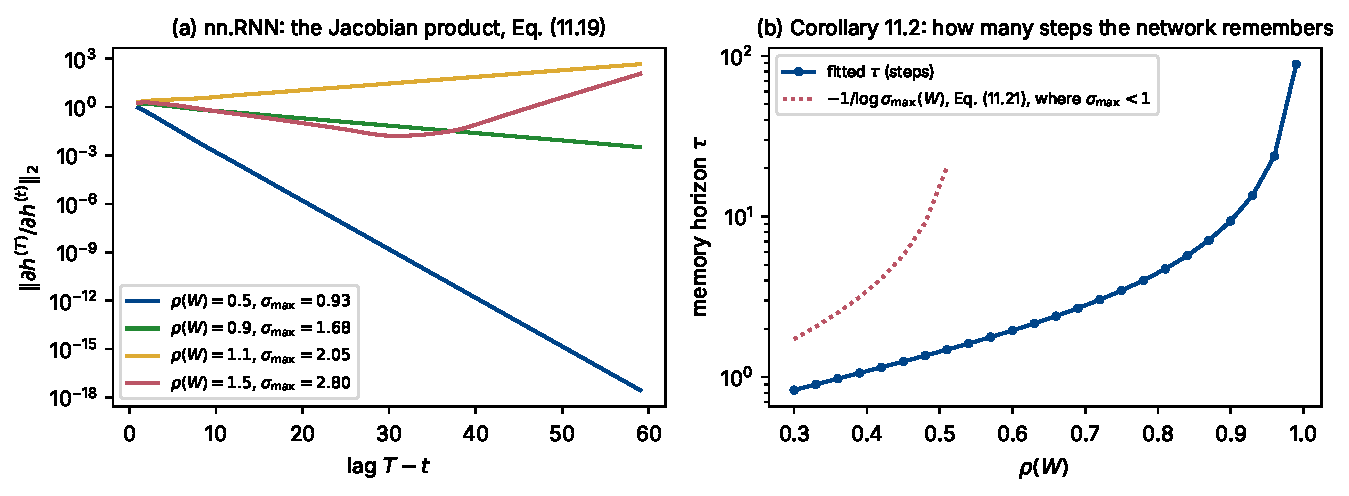
\includegraphics[width=0.8\textwidth]{week45_gradients}
\end{center}
\small
$n_h=20$, $T=60$, inputs small enough that $\tanh'\approx1$, $\bm{W}$ scaled
to a prescribed spectral radius; each curve is
\texttt{torch.autograd.functional.jacobian} of $\bm{h}^{(T)}$ with respect to
$\bm{h}^{(t)}$.  (a) At $\rho(\bm{W})=0.5$ the influence of the first step on
the last has fallen by \emph{eighteen orders of magnitude} over $59$ steps.
At $\rho=1.1$ it has grown to $450$.  (b) The horizon $\tau$ fitted to the
slope of (a): below one step at $\rho=0.3$, ninety at $\rho=0.99$.
\end{frame}

\begin{frame}[fragile]{The numbers behind the figure}
\begin{lstlisting}
 rho(W)  sigma_max  mean max(tanh')   ||dh_T/dh_1||   bound sigma_max^59   fitted tau
  0.50     0.933        1.0000          2.878e-18        1.705e-02           1.44
  0.90     1.680        1.0000          3.313e-03        1.963e+13           9.38
  1.10     2.053        1.0000          4.547e+02        2.721e+18         -10.63
  1.50     2.800        0.9980          1.152e+02        2.410e+26         -20.40

 fitted memory horizon and the lag at which the influence has fallen by 1e-6:
   rho=0.50  tau=  1.44 steps   lag(1e-6)=  20
   rho=0.70  tau=  2.79         lag(1e-6)=  39
   rho=0.90  tau=  9.38         lag(1e-6)= 130
   rho=0.99  tau= 88.88         lag(1e-6)=1228
\end{lstlisting}
\small
The code that produced this is a dozen lines of the notebook: build the
layer, scale \texttt{weight\_hh\_l0}, run it, and ask autograd for the
Jacobian from each intermediate state to the last.
\end{frame}

\begin{frame}{Reading the table}
\begin{itemize}
  \item At $\rho(\bm{W})=0.5$ the memory horizon is \emph{one and a half
        steps}.  A network initialised this way has forgotten its input
        after two steps, and no amount of training on long sequences will
        change that until the weights themselves grow.
  \item The bound uses $\sigma_{\max}(\bm{W})$, not $\rho(\bm{W})$, and the
        two differ: $\rho=0.5$ has $\sigma_{\max}=0.93$, $\rho=0.9$ has
        $\sigma_{\max}=1.7$.  Between $\rho<1<\sigma_{\max}$ there is a
        regime of \emph{transient growth with asymptotic decay} -- the
        red curve of (a).  That is where carefully initialised recurrent
        networks actually operate.
  \item None of this depends on the library.  Autograd computes the product
        of Eq.~(11.19) exactly; the vanishing gradient is \emph{a property
        of the composition}, not of an implementation.
\end{itemize}
\end{frame}

\begin{frame}{Two bits per step, and one per cent from the edge}
\begin{itemize}
  \item The logistic function has $\max|\sigma'|=1/4$ ($\sigma'=\sigma(1-\sigma)$
        at $\sigma=1/2$); $\tanh$ has $\max|\tanh'|=1$ at the origin.  A
        logistic recurrence shrinks the gradient by at least $4^{T-t}$ over a
        lag $T-t$ whatever $\bm{W}$ does -- two bits per step, $10^{35}$ over
        sixty steps.
  \item With $\tanh$, $\tau=-1/\log\sigma_{\max}$: $9.5$ steps at
        $\sigma_{\max}=0.9$, $99.5$ at $0.99$, $999.5$ at $0.999$.  A
        horizon of $100$ steps needs $\sigma_{\max}\ge e^{-1/100}\approx0.990$.
  \item The growth condition of the theorem is $\mu\sigma_{\max}>1$, and
        $0.99$ sits one per cent below it.  To remember a hundred steps the
        simple RNN must be tuned to within a per cent of the exploding
        regime -- and training moves $\bm{W}$.
\end{itemize}
\medskip
That is the design problem the gated cells of next Monday solve.  Today:
what the simple cell can do when the sequences are short enough, and the
one remedy that is free.
\end{frame}


\begin{frame}{Gradient clipping, Eq.~(11.23)}
Vanishing and exploding gradients are not symmetric problems.  Explosion is
the easier of the two, because it is \emph{visible}: the gradient norm
spikes and the parameters jump.  The standard fix rescales any gradient
whose norm exceeds a threshold, keeping the direction:
\[
  \bm{g}\longleftarrow
  \begin{cases}
    \bm{g}, & \|\bm{g}\|\le\theta,\\[2pt]
    \dfrac{\theta}{\|\bm{g}\|}\,\bm{g}, & \|\bm{g}\|>\theta.
  \end{cases}
\]
\begin{block}{Proposition 11.3: clipping is a trust region}
(i) $\tilde{\bm{g}}=\lambda\bm{g}$ with $\lambda\in(0,1]$, so
$-\tilde{\bm{g}}$ is still a descent direction.  (ii) $\tilde{\bm{g}}$ is
the projection of $\bm{g}$ onto the ball of radius $\theta$, Eq.~(11.24),
so a step $\gamma\tilde{\bm{g}}$ never moves the parameters further than
$\gamma\theta$ -- the guarantee of a trust-region method, for free.
\end{block}
\end{frame}

\begin{frame}{Clipping: what it does not do, and where it lives}
\begin{block}{What it does not do}
Nothing whatever for \emph{vanishing} gradients: rescaling $10^{-18}$
upwards would amplify rounding noise, not signal.  Vanishing gradients need
a change of architecture -- the gated cells of next Monday.
\end{block}
\begin{block}{In the libraries}
\texttt{Adam(lr, clipnorm=1.0)} in Keras;
\texttt{nn.utils.clip\_grad\_norm\_(model.parameters(), 1.0)} between
\texttt{backward()} and \texttt{step()} in PyTorch.  Both act on the
\emph{whole} gradient vector, all arrays jointly.
\end{block}
\begin{block}{Initialisation}
$\sigma_{\max}(\bm{W})\approx1$ puts the network at the edge between the
two regimes -- the best this architecture can do.  Orthogonal or identity
initialisations of $\bm{W}$ are attempts to sit exactly there.
\end{block}
\end{frame}

\begin{frame}{Four effective ways to train a recurrent network}
\begin{enumerate}
  \item \textbf{Long short-term memory.}  Make the RNN out of modules
        designed to remember values for a long time -- next Monday.
  \item \textbf{Hessian-free optimisation.}  An optimiser that can detect
        directions with a tiny gradient but an even smaller curvature
        (Newton's method of week 37 made affordable).
  \item \textbf{Echo-state networks.}  Initialise the recurrent
        connections very carefully, so that the hidden state is a reservoir
        of weakly coupled oscillators -- and learn only the read-out $\bm{V}$
        (linear regression, week 35!).
  \item \textbf{Good initialisation with momentum.}  Initialise as in an
        echo-state network, then learn everything, with momentum and
        clipping.
\end{enumerate}
\medskip
In practice: a gated cell, $\sigma_{\max}(\bm{W})\approx1$ at the start,
Adam, and clipping.  Before we gate anything, let us see what the plain
layer can do when the sequences are short enough.
\end{frame}

\begin{frame}[fragile]{The oscillator experiment, 1: the data and the Keras model (Section 11.6.1)}
\begin{lstlisting}
def make_windows(x, L=40, stride=5):           # x: one trajectory of 800 points
    idx = range(0, len(x) - L - 1, stride)
    X = np.stack([x[i:i + L] for i in idx])[..., None]        # (152, 40, 1): inputs x_i..x_{i+39}
    Y = np.stack([x[i + 1:i + L + 1] for i in idx])[..., None] # (152, 40, 1): targets, one step ahead
    return X, Y

model = keras.Sequential([keras.Input(shape=(None, 1)),
                          layers.SimpleRNN(24, return_sequences=True),
                          layers.Dense(1)])
model.compile(optimizer=keras.optimizers.Adam(5e-3, clipnorm=1.0), loss="mse")
model.fit(X_train, Y_train, epochs=300, batch_size=4, verbose=0)
\end{lstlisting}
\small
\begin{itemize}
  \item Data: the \emph{single} RK4 trajectory of panel (a), $\eta=0.2$,
        $(x_0,v_0)=(1,0)$, $800$ points -- the network sees only $x(t)$.
  \item Task: one-step-ahead forecasting at every step, along $152$
        overlapping windows of length $40$ (stride $5$).
  \item Network: $n_h=24$, $649$ parameters; Adam at $5\cdot10^{-3}$,
        clipping at $1$, $300$ epochs.
\end{itemize}
\end{frame}

\begin{frame}[fragile]{The oscillator experiment, 2: the same in PyTorch}
\begin{lstlisting}
model = Forecaster()                       # nn.RNN(1, 24) + nn.Linear(24, 1) from Part 4
opt, lossfn = torch.optim.Adam(model.parameters(), lr=5e-3), nn.MSELoss()
gnorms = []
for epoch in range(300):
    for idx in torch.randperm(len(X_train)).split(4):
        opt.zero_grad()
        loss = lossfn(model(X_train[idx]), Y_train[idx])
        loss.backward()
        gnorms.append(float(nn.utils.clip_grad_norm_(model.parameters(), 1.0)))
        opt.step()
\end{lstlisting}
\small
\begin{block}{The tests}
(b) the trajectory from $(0,1)$ -- a different solution of the same
equation, out of phase with everything the network saw; (c) an oscillator
driven by $F(t)=0.3\cos(0.7t)$ from $(0.5,-0.3)$, which the network never saw
in any form.  The split is by whole trajectories: every test trajectory has
a new initial condition.
\end{block}
\end{frame}

\begin{frame}{Two rules for sequential data}
\begin{block}{No shuffling across time}
Training and test \emph{windows} may be shuffled, the points inside a
window may not -- shuffling in time decorrelates the series and leaks the
future into the past.  \texttt{randperm(...).split(4)} and Keras's
\texttt{shuffle=True} shuffle windows, never steps.
\end{block}
\begin{block}{The cost}
Mean squared error of predicted against actual trajectory, Eq.~(11.5): a
forecasting problem is a regression problem, and we are free to choose
among the regression losses of week 35.
\end{block}
\end{frame}

\begin{frame}[fragile]{The result (\texttt{week45\_oscillator.pdf})}
\begin{center}
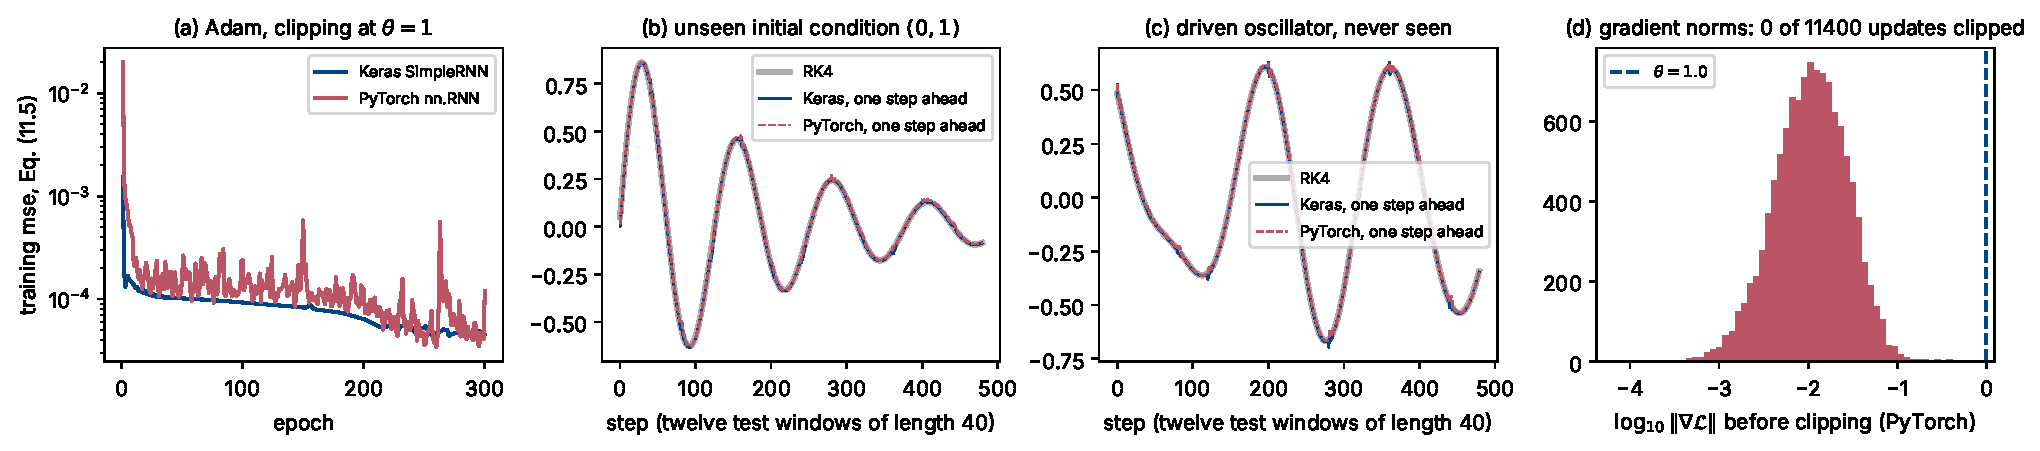
\includegraphics[width=0.95\textwidth]{week45_oscillator}
\end{center}
\begin{lstlisting}
 set          Keras mse   PyTorch mse   Var(x)   relative (Keras / PyTorch)
 train       3.692e-05    1.056e-04   0.0655   0.056% / 0.161%
 unseen IC   3.811e-05    1.023e-04   0.0618   0.062% / 0.166%
 driven      4.970e-05    1.269e-04   0.1488   0.033% / 0.085%
 PyTorch gradient norms before clipping: median 0.011, max 0.77, 0 of 11400 updates clipped
\end{lstlisting}
\end{frame}

\begin{frame}{What the result says}
\begin{itemize}
  \item The second row is the interesting one: trained on a trajectory
        starting from rest at unit displacement, tested on one starting from
        the origin at unit velocity, the error is \emph{the same as the
        training error} -- six parts in ten thousand of the variance in
        Keras, sixteen in PyTorch.
  \item The driven oscillator, never seen, is predicted just as well.
  \item The network has not memorised a trajectory; it has learned the
        \emph{update rule}, as Eq.~(11.12) said it would -- the same payoff
        parameter sharing gave in week 44: a rule learned once applies
        everywhere it is valid.
  \item The two libraries differ by a factor of three in the final error:
        different random initialisations and different batch orderings.
        Both are far below anything that matters.
  \item (d): with $\sigma_{\max}(\bm{W})\approx1$ at the start and sequences
        of $40$ steps, clipping never fired in $11\,400$ updates.  It is
        insurance.
\end{itemize}
\end{frame}


%% =====================================================================
\section{Three applications}


\begin{frame}[fragile]{Forecasting a sine wave, 1: Keras (Section 11.8.1)}
\begin{lstlisting}
time_steps = np.linspace(0, 100, 500); data = np.sin(time_steps); seq_length = 20
X = np.array([data[i:i+seq_length] for i in range(len(data)-seq_length)]).reshape(-1, seq_length, 1)
y = data[seq_length:].reshape(-1, 1)                       # the next value after each window
split = int(0.8 * len(X))                                  # split in TIME, not at random

model = keras.Sequential([keras.Input(shape=(seq_length, 1)),
                          layers.SimpleRNN(16),            # last state only: (N, 16)
                          layers.Dense(1)])
model.compile(optimizer=keras.optimizers.Adam(1e-2, clipnorm=1.0), loss="mse")
model.fit(X[:split], y[:split], epochs=200, batch_size=32, verbose=0,
          validation_data=(X[split:], y[split:]))
\end{lstlisting}
\small
Sequence-to-label: $20$ values in, \emph{one} value out, so
\texttt{return\_sequences} stays at its default \texttt{False} and
\texttt{Dense(1)} acts on the last state.  The last $20\%$ of the wave is
the test set.
\end{frame}

\begin{frame}[fragile]{Forecasting a sine wave, 2: PyTorch}
\begin{lstlisting}
class SineRNN(nn.Module):
    def __init__(self, hidden=16):
        super().__init__()
        self.rnn = nn.RNN(input_size=1, hidden_size=hidden, batch_first=True)
        self.fc = nn.Linear(hidden, 1)
    def forward(self, x):
        out, h_T = self.rnn(x)                 # out: (N, 20, 16), every h_t
        return self.fc(out[:, -1, :])          # read out the last state only

model = SineRNN(); opt = torch.optim.Adam(model.parameters(), lr=1e-2); lossfn = nn.MSELoss()
for epoch in range(200):
    for idx in torch.randperm(split).split(32):
        opt.zero_grad()
        loss = lossfn(model(X[idx]), y[idx])
        loss.backward()
        nn.utils.clip_grad_norm_(model.parameters(), 1.0)
        opt.step()
\end{lstlisting}
\small
\texttt{out[:, -1, :]} is Keras's \texttt{return\_sequences=False}.  The
loop is the one of Part 4, unchanged.
\end{frame}

\begin{frame}[fragile]{Both reach the same place (\texttt{week45\_sine.pdf})}
\begin{center}
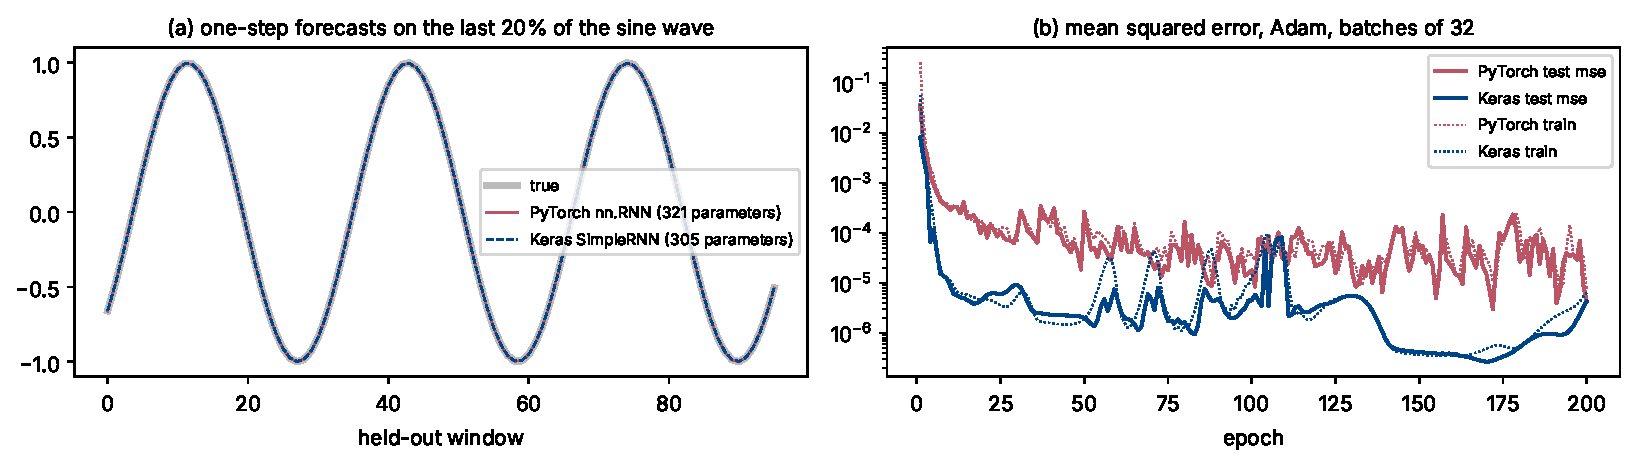
\includegraphics[width=0.9\textwidth]{week45_sine}
\end{center}
\begin{lstlisting}
PyTorch    epoch 200: train mse 0.000008   test mse 0.000004   (321 parameters)
Keras      epoch 200: train mse 0.000006   test mse 0.000004   (305 parameters)
rms error on the held-out windows: 0.0021 (both), amplitude 1
\end{lstlisting}
\small
A test mean squared error of a few $10^{-6}$ is a root-mean-square error of
a few $10^{-3}$ on a signal of unit amplitude: both predictions lie on the
true curve.  The parameter counts differ by sixteen: the second bias vector.
\end{frame}

\begin{frame}[fragile]{MNIST read row by row (Section 11.8.2)}
Treat each $28\times28$ image as a sequence of $28$ rows, each of $28$
features, and classify it from the last state -- a sequence-to-label task.
Not what one does in practice (the recap said why a CNN is the right tool),
but a clean demonstration, and a direct comparison with week 44.
\begin{lstlisting}
# Keras
m = keras.Sequential([keras.Input(shape=(28, 28)), layers.SimpleRNN(128), layers.Dense(10)])
m.compile(optimizer=keras.optimizers.Adam(1e-3, clipnorm=1.0),
          loss=keras.losses.SparseCategoricalCrossentropy(from_logits=True), metrics=["accuracy"])
m.fit(x_train, y_train, epochs=3, batch_size=64)        # x_train: (60000, 28, 28) in [0, 1]

# PyTorch
class RowNet(nn.Module):
    def __init__(self):
        super().__init__()
        self.rnn = nn.RNN(28, 128, batch_first=True)     # 28 steps of 28 features
        self.fc = nn.Linear(128, 10)
    def forward(self, x):
        return self.fc(self.rnn(x)[0][:, -1, :])         # last state -> class scores
criterion = nn.CrossEntropyLoss()                        # softmax + cross entropy, week 41
\end{lstlisting}
\small Compare the CNN program of the recap: the same \texttt{Input} -- layer
-- \texttt{Dense(10)} pattern, the same loss, the same loop; only the layer
in the middle has changed, and with it the way the image is read.
\end{frame}

\begin{frame}[fragile]{Row by row: the result (\texttt{week45\_mnist\_rows.pdf})}
\begin{columns}[T]
\begin{column}{0.5\textwidth}
\begin{center}
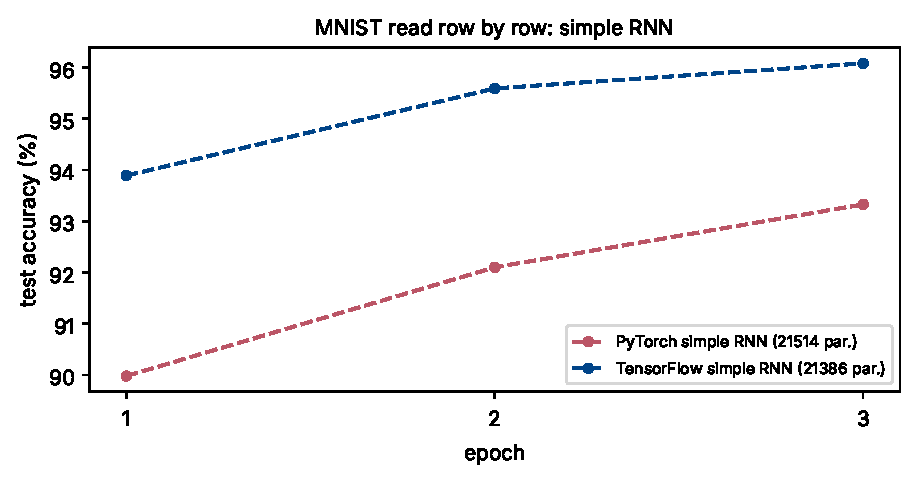
\includegraphics[width=\textwidth]{week45_mnist_rows}
\end{center}
\end{column}
\begin{column}{0.5\textwidth}
\begin{lstlisting}
cell        framework   parameters  test acc.
simple RNN  PyTorch          21514     0.9333
simple RNN  Keras            21386     0.9608
(CNN, week 44               3241354     0.9906)
\end{lstlisting}
\small Three epochs, Adam $10^{-3}$, batches of $64$, $n_h=128$, the full
$60\,000$ images; accuracy on the $10\,000$ test images.
\end{column}
\end{columns}
\begin{itemize}
  \item A simple recurrent layer with $21\,000$ parameters reads the image
        in $28$ steps and gets $93$--$96\%$: the task is within its memory
        horizon, and the parameter count is again independent of the image
        height.
  \item The CNN of the recap reached $99\%$: reading an image as a sequence
        throws away the vertical structure that convolution was built to
        exploit.  The right tool for images is still the CNN; the point here
        is that the recurrent layer is a drop-in replacement in the code.
\end{itemize}
\end{frame}

\begin{frame}{The experiment the theory demands: the adding problem (Section 11.8.5)}
Corollary 11.2 says a simple RNN initialised in the usual way has a memory
horizon of a few steps.  MNIST rows and the oscillator windows were short
enough.  Testing the claim needs a task where nothing but long-range memory
is measured.
\begin{block}{The adding problem}
Each sequence has two channels: the first carries values drawn uniformly
from $[0,1]$, the second is zero except for exactly two markers, one in
each half.  The target is half the sum of the two marked values.
\end{block}
Nothing can be inferred from local statistics -- the values are i.i.d.\ --
so a model must hold one number from the first half until the second marker
arrives, while ignoring everything in between.  Predicting the mean gives
a mean squared error of about $0.043$; that is the number to beat.
\end{frame}

\begin{frame}[fragile]{The adding problem: setup}
\begin{lstlisting}
for T in (10, 30, 60, 120):
    core, head = nn.RNN(2, 32, batch_first=True), nn.Linear(32, 1)   # two channels in
    params = list(core.parameters()) + list(head.parameters())
    opt = torch.optim.Adam(params, lr=5e-3)
    for epoch in range(40):
        for idx in torch.randperm(3000).split(64):
            opt.zero_grad()
            loss = nn.MSELoss()(head(core(X[idx])[0][:, -1, :]), y[idx])
            loss.backward(); nn.utils.clip_grad_norm_(params, 1.0); opt.step()
\end{lstlisting}
\small
\begin{itemize}
  \item $3000$ training and $1000$ held-out sequences; $n_h=32$; the same
        seed, optimiser and epochs for every $T$.
  \item Sequence-to-label again: the read-out sees \texttt{[0][:, -1, :]},
        the last state.
  \item Prediction from Corollary 11.2: a dependency at lag $30$ should be
        invisible to this network.
\end{itemize}
\end{frame}

\begin{frame}[fragile]{Where the horizon runs out (\texttt{week45\_adding.pdf})}
\begin{columns}[T]
\begin{column}{0.5\textwidth}
\begin{center}
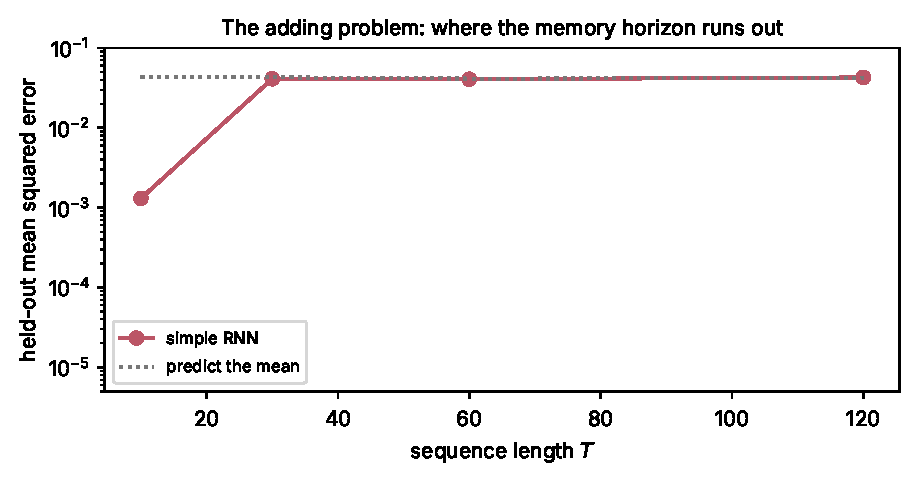
\includegraphics[width=\textwidth]{week45_adding}
\end{center}
\end{column}
\begin{column}{0.5\textwidth}
\begin{lstlisting}
   T   baseline   simple RNN
  10     0.0427       0.0013
  30     0.0429       0.0410
  60     0.0411       0.0405
 120     0.0425       0.0426
\end{lstlisting}
\small Held-out mean squared error; the baseline column is predicting the
mean.
\end{column}
\end{columns}
\begin{itemize}
  \item At $T=10$ the simple recurrent network solves the task: $0.0013$
        against $0.0427$.
  \item At $T=30$ it has \emph{already failed completely} -- an error equal
        to the baseline is a model that outputs the mean and nothing else --
        and it never recovers at $60$ or $120$.  The gap between $T=10$ and
        $T=30$ is where the horizon of Corollary 11.2 runs out.
  \item Next Monday we change the cell, keep everything else in this code,
        and run the same table again.
\end{itemize}
\end{frame}

%% =====================================================================
\begin{frame}{Where this is going: tomorrow, Project 2, next week}
\begin{columns}[T]
\begin{column}{0.5\textwidth}
\begin{block}{Tomorrow: Project 2}
The Tuesday session is yours for Project 2 (deadline \textbf{Monday
November 9}): open questions first, then work in your groups with us
circulating.  Bring your results and the parts of the report you are
unsure about.  No weekly exercises this week.
\end{block}
\begin{block}{If you want to use today in Project 2}
You do not have to.  A group that treats the regression part as a
one-step forecasting problem -- the Runge function sampled along $x$ as a
sequence -- and compares a Keras or PyTorch recurrent network against its
dense network is welcome to, cross-validated the same way and compared
honestly.
\end{block}
\end{column}
\begin{column}{0.48\textwidth}
\begin{block}{Reading}
Chapter 11, Sections 11.1--11.6 and 11.8 (11.7 is next week); Goodfellow et
al.\ Chapter 10; Raschka et al.\ Chapter 15.  The code of today is in
\texttt{week45.ipynb}.
\end{block}
\begin{block}{Next Monday, week 46}
First hour: the gated cells -- long short-term memory and the gated
recurrent unit, Section 11.7 -- measured the same way, run on the adding
problem, and on sound (spoken digits).  Then decision trees and ensemble
methods (Chapter 7).
\end{block}
\end{column}
\end{columns}
\end{frame}

\begin{frame}{Summary of week 45}
\small
\begin{block}{From convolution to recurrence}
A CNN shares its parameters along the spatial axes; a recurrent network
shares them along the time axis.  The simple RNN is a learned dynamical
system -- the oscillator showed it is a learned time-stepping scheme -- and
in the libraries it is one layer, \texttt{SimpleRNN} or \texttt{nn.RNN},
fed a 3-tensor \texttt{(samples, timesteps, features)}, in the same
\texttt{Sequential} / training-loop pattern as the CNN.
\end{block}
\begin{block}{How it is trained, and why that is hard}
\texttt{loss.backward()} and \texttt{model.fit} perform backpropagation
through time exactly: a linear backward pass whose gradient across a lag is
a product of Jacobians -- $10^{-18}$ over $59$ steps at $\rho(\bm{W})=0.5$,
a memory horizon of $1.4$ steps, measured with autograd.  Clipping handles
explosion for free and does nothing for vanishing.
\end{block}
\begin{block}{What the simple cell can and cannot do}
Trained on one damped oscillation it predicted an unseen initial condition
and an unseen forcing at the training error: it learned the rule, not the
trajectory.  It reads MNIST in $28$ steps at $93$--$96\%$.  And on the
adding problem it fails from $T=30$ -- exactly where Corollary 11.2 says
its memory runs out.  Next Monday: the cell that does not.
\end{block}
\end{frame}

\end{document}
